\documentclass[a4paper, 12pt]{article}
\usepackage[margin=1in]{geometry}
\usepackage{graphicx}
\usepackage{amsmath, amsthm, amssymb, amsfonts}
\usepackage{fancyhdr}
\usepackage{tikz}
\usepackage{parskip}
\usepackage{float}
\usepackage{enumitem}
\usepackage{array}
\usepackage[labelsep=none, labelfont=bf]{caption}


\usetikzlibrary{automata, positioning, arrows}

\setlength{\headheight}{14.49998pt}

\tikzset {
    ->,
    >=stealth',
    node distance=3.5cm,
    every state/.style={thick, fill=gray!10},
    initial text = $ $
}

\makeatletter
\renewenvironment{proof}[1][\proofname]{\par
%  \pushQED{\qed}% <--- remove the QED business
  \normalfont \topsep6\p@\@plus6\p@\relax
  \trivlist
  \item[\hskip\labelsep
        \itshape
    #1\@addpunct{.}]\ignorespaces
}{%
%  \popQED% <--- remove the QED business
  \endtrivlist\@endpefalse
}
\renewcommand\qedhere{} % to ensure code portability
\makeatother

\pagestyle{fancy}
\fancyhead[l]{SECJ3203}
\fancyhead[c]{Tutorial 9}
\fancyhead[r]{1 June 2025}

\title{Tutorial 9 & 10}
\date{}
\author{}

\renewcommand{\proofname}{Solution:}

\begin{document}
    \begin{enumerate}
        \item Let $M$ be the Turing machine defined by Table 1 where the start and final states are $q_0$ and $q_2$, respectively.

        \begin{table}[ht]
            \centering
            \caption{}
            \begin{tabular}{|c|c|c|c|}
                \hline
                $\delta$ & $B$ & $a$ & $b$ \\ \hline
                $q_0$ & $q_1, B, R$ & - & - \\ \hline
                $q_1$ & $q_2, B, R$ & $q_1, 0, R$ & $q_1, 1, R$ \\ \hline
                $q_2$ & - & - & - \\
                \hline
            \end{tabular}
            \caption*{\small \textbf{Note:} $B$ -- blank symbol}
        \end{table}
        \begin{enumerate}
            \item Give the state diagram of $M$.
                \begin{proof}
                    \leavevmode
                    
                    \begin{center}
                        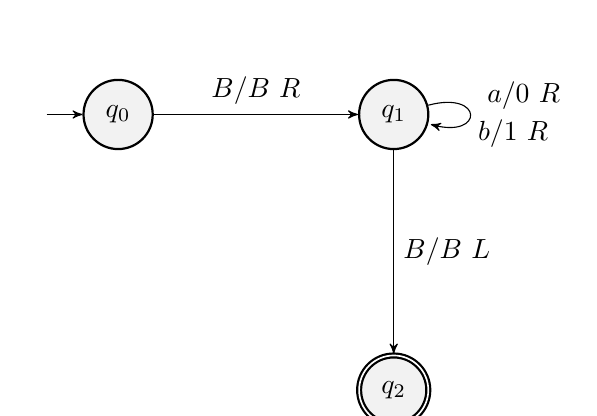
\begin{tikzpicture}
                            \node[state, initial] (q0) {$q_0$};
                            \node[state, right of=q0] (q1) {$q_1$};
                            \node[state, accepting, below of=q1] (q2) {$q_2$};

                            \draw
                             (q0) edge[above] node{$B/B \ R$} (q1)
                             (q1) edge[right] node{$B/B \ L$} (q2)
                             (q1) edge[loop right] node[pos=0.6, above, xshift=20]{$a/0 \ R$} node[pos=0.6, yshift=-5]{$b/1 \ R$} (q1);
                        \end{tikzpicture}
                    \end{center}
                \end{proof}
            \item Trace the computation for the input string $aabba$.
                \begin{proof}
                    \begin{align*}
                        q_0BaabbaB &\vdash Bq_1aabbaB \\
                        &\vdash B0q_1abbaB \\
                        &\vdash B00q_1bbaB \\
                        &\vdash B001q_1baB \\
                        &\vdash B0011q_1aB \\
                        &\vdash B00110q_1B \\
                        &\vdash B0011q_20B
                    \end{align*}
                \end{proof}
            \item Trace the computation for the input string $baba$.
                \begin{proof}
                    \begin{align*}
                        q_0BbabaB &\vdash Bq_1babaB \\
                        &\vdash B1q_1abaB \\
                        &\vdash B10q_1baB \\
                        &\vdash B101q_1aB \\
                        &\vdash B1010q_1B \\
                        &\vdash B101q_20B
                    \end{align*}
                \end{proof}
            \item Describe the result of a computation in $M$.
                \begin{proof}
                    The computation in $M$ maps every $a$ in the input string to $0$, and every $b$ to 1.
                \end{proof}
        \end{enumerate}

        \item Let $M$ be the Turing Machine diagram as follows:
        \begin{center}
            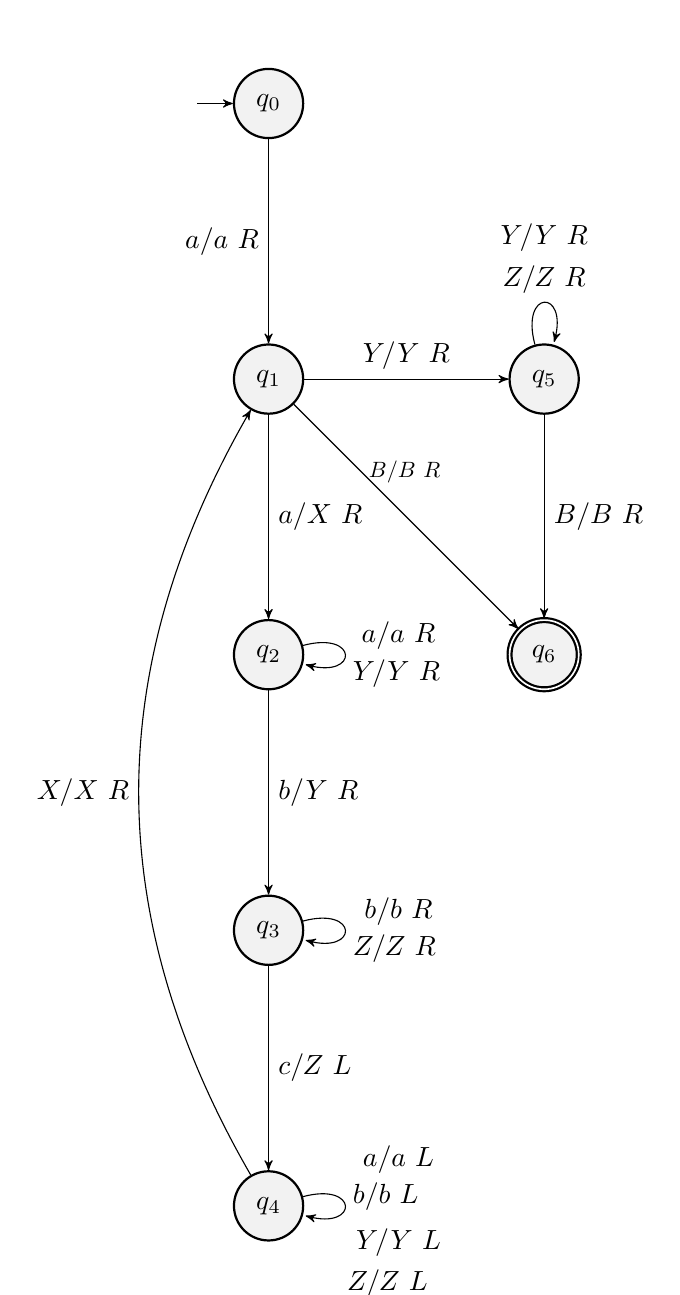
\begin{tikzpicture}
                \node[state, initial] (q0) {$q_0$};
                \node[state, below of=q0] (q1) {$q_1$};
                \node[state, below of=q1] (q2) {$q_2$};
                \node[state, below of=q2] (q3) {$q_3$};
                \node[state, below of=q3] (q4) {$q_4$};
                \node[state, right of=q1] (q5) {$q_5$};
                \node[state, accepting, below of=q5] (q6) {$q_6$};

                \draw
                (q0) edge[left] node{$a/a \ R$} (q1)
                (q1) edge[right] node{$a/X \ R$} (q2)
                (q1) edge[above] node{$Y/Y \ R$} (q5)
                (q1) edge[right] node[pos=0.3, scale=0.8]{$B/B \ R$} (q6)
                (q2) edge[right] node{$b/Y \ R$} (q3)
                (q2) edge[loop right] node[pos=0.6, above, xshift=20] {$a/a \ R$} node[pos=0.6, yshift=-5]{$Y/Y \ R$} (q2)
                (q3) edge[right] node{$c/Z \ L$} (q4)
                (q3) edge[loop right] node[pos=0.6, above, xshift=20] {$b/b \ R$} node[pos=0.6, yshift=-5]{$Z/Z \ R$} (q3)
                (q4) edge[loop right] node[pos=0.6, above, xshift=20, yshift=10] {$a/a \ L$} node[pos=0.6,  yshift=5]{$b/b \ L$} node[pos=0.6, above, xshift=20, yshift=-20]{$Y/Y \ L$} node[pos=0.6, above, xshift=16, yshift=-35]{$Z/Z \ L$}  (q4)
                (q4) edge[bend left] node[left]{$X/X \ R$} (q1)
                (q5) edge[right] node{$B/B \ R$} (q6)
                (q5) edge[loop above] node[pos= 0.5, yshift = 15]{$Y/Y \ R$} node[pos=0.5]{$Z/Z \ R$} (q5);
            \end{tikzpicture}
        \end{center}
        \begin{enumerate}
            \item Give the transition table of $M$.
                \begin{proof}
                    \leavevmode
                    \begin{table}[H]
                        \centering
                        \begin{tabular}{|c|c|c|c|c|c|c|c|c|}
                            \hline
                            $\delta$ & $B$ & $a$ & $b$ & $c$ & $X$ & $Y$ & $Z$ \\ \hline
                            $q_0$ & - & $q_1, a, R$ & - & - & - & - & - \\ \hline
                            $q_1$ & $q_6, B, R$ & $q_2, X, R$ & - & - & - & $q_5, Y, R$ & - \\ \hline 
                            $q_2$ & - & $q_2, a, R$ & $q_3, Y, R$ & - & - & $q_2, Y, R$ & - \\ \hline
                            $q_3$ & - & - & $q_3, b, R$ & $q_4, Z, L$ & - & - & $q_3, Z, R$ \\ \hline
                            $q_4$ & - & $q_4, a, L$ & $q_4, b, L$ & - & $q_1, X, R$ & $q_4, Y, L$ & $q_4, Z, L$ \\ \hline
                            $q_5$ & $q_6, B, R$ & - & - & - & - & $q_5, Y, R$ & $q_5, Z, R$ \\ \hline
                            $q_6$ & - & - & - & - & - & - & - \\ \hline 
                        \end{tabular}
                    \end{table}
                \end{proof}
            \item Trace the computations of $M$ on input strings $abc$ and $aabc$.
                \begin{proof}
                
                    $abc:$
                    \begin{align*}
                        &q_0abc \vdash aq_1bc \\
                        &\text{No transitions, machine halts...}
                    \end{align*}

                    $aabc$:
                    \begin{align*}
                        q_0aabc &\vdash aq_1abc \\
                        &\vdash aXq_2bc \\
                        &\vdash aXYq_3c \\
                        &\vdash aXq_4YZ \\
                        &\vdash aq_4XYZ \\
                        &\vdash aXq_1YZ \\
                        &\vdash aXYq_5Z \\
                        &\vdash aXYZq_5B \\
                        &\vdash aXYZBq_6B
                    \end{align*}
                \end{proof}
            \item Give a set-theoretic definition to define the language.
                \begin{proof}
                    $L(M)=\{a^{n+1}b^nc^n \mid n \geq 0\}$
                \end{proof}
        \end{enumerate}
    \end{enumerate}

    \newpage
    \fancyhead[c]{Tutorial 10}

    \begin{enumerate}
        \item 
        Given the languages, $L$ as follows in Table 1. For each languages answer questions (a) - (b):
        \setcounter{table}{0}
        \begin{table}[ht]
            \centering
            \caption{}
            \begin{tabular}{|c|}
                \hline
                \textbf{Languages} \\ \hline
                i. $L = \{a^{m+1}b^mc^n \mid m=n \ \text{and} \ m, n \geq0\}$ \\ \hline
                ii. $L=\{a^{m+1}b^nc^{2m} \mid m, n \geq 0\}$ \\ \hline
            \end{tabular}
        \end{table}
        \begin{enumerate}
            \item Design the Turing Machine that accept the language $L(M)$.
                \begin{proof}
                \leavevmode
                    \begin{figure}[H]
                        \centering
                        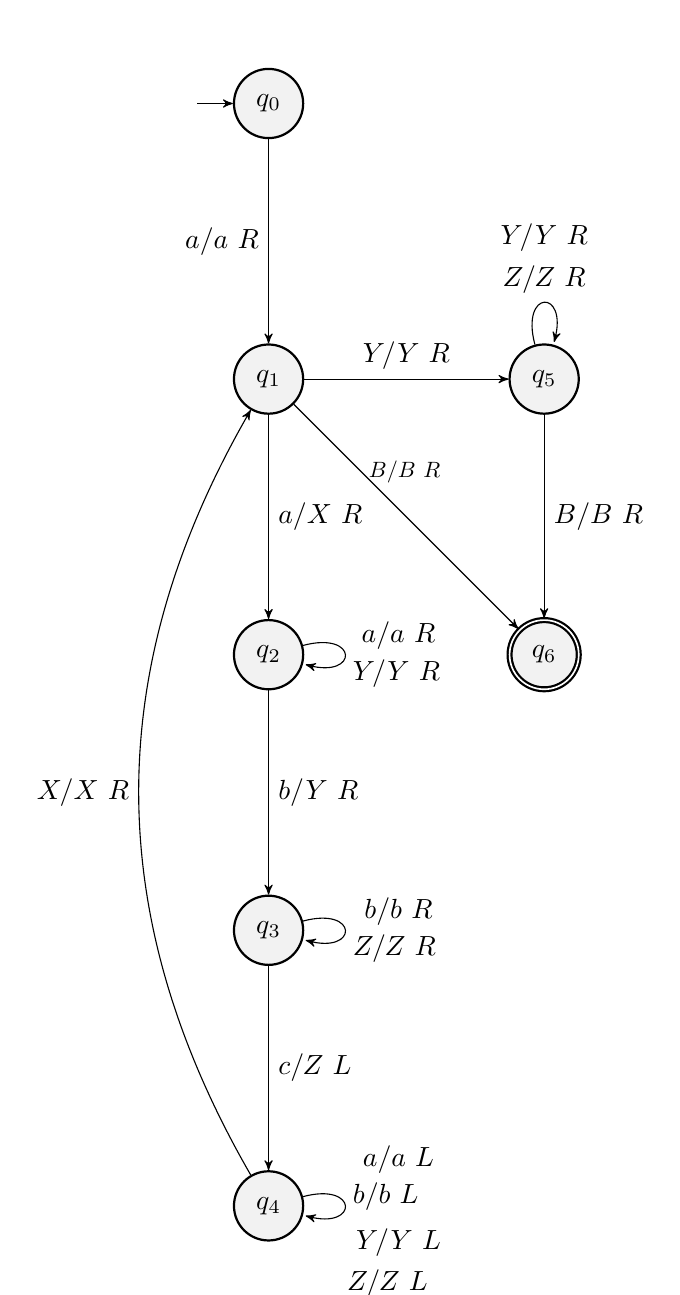
\begin{tikzpicture}
                            \node[state, initial] (q0) {$q_0$};
                            \node[state, below of=q0] (q1) {$q_1$};
                            \node[state, below of=q1] (q2) {$q_2$};
                            \node[state, below of=q2] (q3) {$q_3$};
                            \node[state, below of=q3] (q4) {$q_4$};
                            \node[state, right of=q1] (q5) {$q_5$};
                            \node[state, accepting, below of=q5] (q6) {$q_6$};

                            \draw
                            (q0) edge[left] node{$a/a \ R$} (q1)
                            (q1) edge[right] node{$a/X \ R$} (q2)
                            (q1) edge[above] node{$Y/Y \ R$} (q5)
                            (q1) edge[right] node[pos=0.3, scale=0.8]{$B/B \ R$} (q6)
                            (q2) edge[right] node{$b/Y \ R$} (q3)
                            (q2) edge[loop right] node[pos=0.6, above, xshift=20] {$a/a \ R$} node[pos=0.6, yshift=-5]{$Y/Y \ R$} (q2)
                            (q3) edge[right] node{$c/Z \ L$} (q4)
                            (q3) edge[loop right] node[pos=0.6, above, xshift=20] {$b/b \ R$} node[pos=0.6, yshift=-5]{$Z/Z \ R$} (q3)
                            (q4) edge[loop right] node[pos=0.6, above, xshift=20, yshift=10] {$a/a \ L$} node[pos=0.6,  yshift=5]{$b/b \ L$} node[pos=0.6, above, xshift=20, yshift=-20]{$Y/Y \ L$} node[pos=0.6, above, xshift=16, yshift=-35]{$Z/Z \ L$}  (q4)
                            (q4) edge[bend left] node[left]{$X/X \ R$} (q1)
                            (q5) edge[right] node{$B/B \ R$} (q6)
                            (q5) edge[loop above] node[pos= 0.5, yshift = 15]{$Y/Y \ R$} node[pos=0.5]{$Z/Z \ R$} (q5);
                        \end{tikzpicture}
                        \captionsetup{labelsep=colon, labelfont=bf, labelformat=empty}
                        \caption{$L = \{a^{m+1}b^mc^n \mid m=n \ \text{and} \ m, n \geq0\}$}
                    \end{figure}
                    \begin{figure}[H]
                        \centering
                        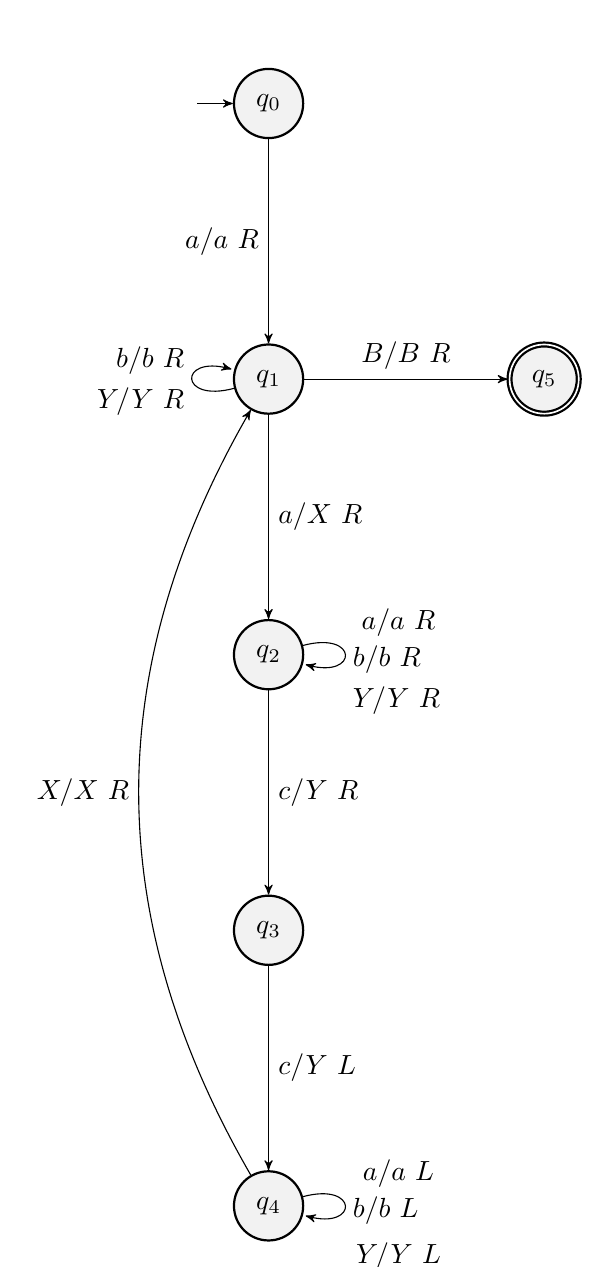
\begin{tikzpicture}
                            \node[state, initial] (q0) {$q_0$};
                            \node[state, below of=q0] (q1) {$q_1$};
                            \node[state, below of=q1] (q2) {$q_2$};
                            \node[state, below of=q2] (q3) {$q_3$};
                            \node[state, below of=q3] (q4) {$q_4$};
                            \node[state, accepting, right of=q1] (q5) {$q_5$};

                            \draw
                            (q0) edge[left] node{$a/a \ R$} (q1)
                            (q1) edge[right] node{$a/X \ R$} (q2)
                            (q1) edge[loop left] node[pos=0.6, yshift = 5]{$b/b \ R$} node[pos=0.6, yshift = -10]{$Y/Y \ R$} (q1)
                            (q1) edge[above] node{$B/B \ R$} (q5)
                            (q2) edge[right] node{$c/Y \ R$} (q3)
                            (q2) edge[loop right] node[pos=0.6, above, xshift=20, yshift=5] {$a/a \ R$} node[pos=0.6, yshift=0]{$b/b \ R$} node[pos=0.6, yshift=-15]{$Y/Y \ R$} (q2)
                            (q3) edge[right] node{$c/Y \ L$} (q4)
                            (q4) edge[loop right] node[pos=0.6, above, xshift=20, yshift=5] {$a/a \ L$} node[pos=0.6,  yshift=0]{$b/b \ L$} node[pos=0.6, above, xshift=20, yshift=-25]{$Y/Y \ L$}  (q4)
                            (q4) edge[bend left] node[left]{$X/X \ R$} (q1);
                        \end{tikzpicture}
                        \captionsetup{labelsep=colon, labelfont=bf, labelformat=empty}
                        \caption{$L = \{a^{m+1}b^nc^{2m} \mid m, n \geq 0\}$}
                    \end{figure}
                \end{proof}
            \item What is the shortest string in the language accepted by the Turing Machine.
                \begin{proof} $ $ \newline
                \leavevmode
                    Shortest string accepted by Language 1: $a$

                    Shortest string accepted by Language 2: $a$
                \end{proof}
        \end{enumerate}
    \end{enumerate}
\end{document}
